
\documentclass{beamer}
\usepackage{HECbeamer}
% \usepackage{pgfpages}
% \pgfpagesuselayout{4 on 1}[letterpaper, landscape, border shrink=5mm]
\title[\color{white}{MATH 60604A \S~4c - Application of logistic regression}]{\texorpdfstring{MATH 60604A \\Statistical modelling \\ \S~4c - Application of logistic regression}{MATH 60604A \\Statistical modelling \\ \S~4c - Application of logistic regression}}
\author{}
\institute{HEC Montréal\\
Department of Decision Sciences}
\date{} 

\begin{document}
\frame{\titlepage}


\begin{frame}[fragile]
\frametitle{Fixation-intention to buy example}

 In the study, subjects navigated a website that contained, among other things, an advertisement for candy. Simultaneously, an ``eye-tracker'' tracked where the subject's eye were fixated on the screen. We can therefore measure whether the subject saw the ad, and for how long. Moreover, a software was used (FaceReader) to measure the facial expressions and infer the emotions of the subject while viewing the ad.
\vp


Suppose that, instead of measuring the intention to buy from the questionnaire, \alert{we had contacted the subjects one month later to see if they had bought the product}.
\end{frame}
\begin{frame}
\frametitle{Number of items bought}
The data includes two variables not considered until now:

\bi\item \code{buy}: a binary variable equal to unity if the subject bought the product and zero otherwise.
\item \texttt{nitem}: integer giving the number of times the item was bought.
\ei
\begin{center}
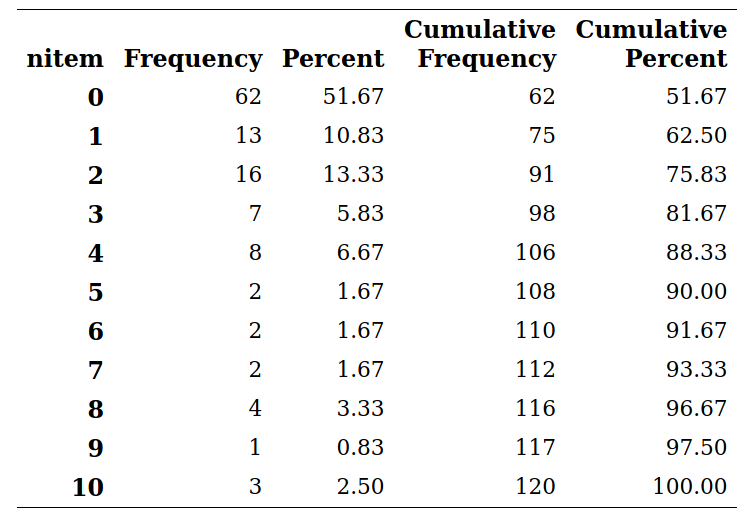
\includegraphics[width = 0.6\linewidth]{img/c4/slides8-e2}
\end{center}
The variable \texttt{nitem} varies from $0$ to $10$ with a mean of $1.71$ purchases per participant. $51.7$\% of the participants did not make any purchase.
\end{frame}

\begin{frame}[fragile]

We focus for now on \texttt{buy} as response. The explanatory variables are as before, namely
 {\small 
\bi
\item \code{fixation}: total duration of fixation on the ad (in seconds).
\item \code{emotion}: measured during the ad fixation, the ratio of the probabilities of having a positive emotion and  of having a negative emotion.
\item \code{sex}: the sex of the subject, zero for male and one for female.
\item \code{age}: the age of the subject (in years).
\item \code{revenue}: annual salary (in dollars), one of 
{ \footnotesize
\be 
\item $[0, 20 000);$
\item $[20 000, 60 000)$; 
\item $60 000$ and above.
\ee
}
\item \code{educ}: the subject's level of education, one of 
{ \footnotesize
\be 
\item high school or lower;
\item college; 
\item university degree.
\ee
}
\item \code{marital}: binary variable giving the marital status, zero for single and one for subjects in a relationship.
\ei
}
\end{frame}
\begin{frame}[fragile]
\frametitle{Logistic model with all the predictor variables}
If we let $\pi=\P{Y=1\mid \mathbf{X}}$ denote the probability of making a purchase given the value of the explanatory variables, the model is

\begin{align*}
\logit(\pi)&=\beta_0 + \beta_1 \code{sex} + \beta_2 \code{age} + \beta_3 \code{revenue}_1 + \beta_4 \code{revenue}_2 \\
&\qquad + \beta_5 \code{educ}_1 + \beta_6 \code{educ}_2 + \beta_7 \code{marital} \\
&\qquad + \beta_8 \code{fixation} + \beta_9 \code{emotion}.
\end{align*}



\end{frame}

\begin{frame}[fragile]
\frametitle{\SASlang code with \code{proc logistic}}
\bi
\item The $\bs{\beta}$ parameters are really only interpretable on the exponential scale.
\item We can use \code{proc logistic} with \code{clparm=pl odds=pl expb} to get exponentiated parameters and confidence intervals.
\item With \code{proc logistic}, the default parametrization for categorical variables is obtained through the option \texttt{param=glm}.
\ei
\begin{tcolorbox}[colback=white, colframe=hecblue, title=\SASlang code with \code{proc logistic}]
\begin{verbatim}
proc logistic data=statmod.intention;
class educ revenue / param=glm;
model buy(ref="0")=sex age revenue educ marital 
    fixation emotion / clparm=pl odds=pl expb;
run;
\end{verbatim}
\end{tcolorbox}
\end{frame}
% 
% \begin{frame}[fragile]
% \frametitle{Coding numerical variables with \code{proc logistic}}
% \bi
% \item Everything we saw in the regression chapter about coding variables through the \code{class} option still applies in the logistic regression framework (and in other kinds of regression models).
% \bi  
% \item since the variables \code{educ} (three levels) and \code{revenue} (three levels) were defined in \code{class}, two indicator variables were included in the model for each.
% \item With \code{proc logistic}, the default parametrization is obtained through
% \begin{tcolorbox}[colback=white, colframe=hecblue, title=SAS code]
% {\small 
% \begin{verbatim}
% proc logistic data=statmod.intention;
% class educ revenue / param=glm;
% [...]
% \end{verbatim}
% }
% \end{tcolorbox}
% \ei
% \ei
% \end{frame}
% \begin{frame}
%  \frametitle{Alternative \SASlang{} formulations using \texttt{glimmix} and \texttt{genmod}}
%  \begin{tcolorbox}[colback=white, colframe=hecblue, title=\SASlang{} code for logistic regression with \texttt{glimmix} and \texttt{genmod}]
% {\small 
% \begin{verbatim}
% proc glimmix data=statmod.intention;
% class educ revenue;
% model buy(ref="0")=sex age revenue educ marital 
%     fixation emotion / dist=binary link=logit solution;
% lsmeans revenue / pdiff=all cl;
% run;
% 
% proc genmod data=statmod.intention;
% class educ revenue;
% model buy=sex age revenue educ marital 
%     fixation emotion / dist=binomial link=logit;
% lsmeans revenue / pdiff=all cl;
% run;
% \end{verbatim}
% \end{tcolorbox}
% \end{frame}

% proc glimmix data=statmod.intention;
% class educ revenue;
% model buy=sex age revenue educ marital 
%     fixation emotion / dist=binomial link=logit solution;
% lsmeans revenue / pdiff=all cl;
% run;
% 


%\begin{tcolorbox}[colback=white, colframe=hecblue, title=SAS code]
%\begin{verbatim}
%proc glimmix data=mydata.reglogistique1;
%class educ revenu;
%model achat(ref="0")=sexe age revenu educ statut 
%    fixation emotion / dist=binary link=logit solution;
%lsmeans revenu / pdiff=all adjust=sidak stepdown cl;
%run;
%\end{verbatim}
%\end{tcolorbox}

% \begin{frame}[fragile]
% \frametitle{Remarks on \SASlang{} specifications}
% \bi
% \item The option \code{dist=binomial} specifies that the response variable is Bernoulli/binomial (with \code{proc glimmix}, one can use \code{dist=binary}).
% \item The option \code{link=logit} specifies that we want the \alert{logit link function}.
% \item The model is fitted using maximum likelihood.
% % \item Note that the response variable \code{buy} was not coded using \code{class} in \SASlang{}, so that it is treated as  numerical. % ONLY FOR PROC GLIMMIX
% \item Check in the log to make sure the following statement appears:
% \verb+procedure is modeling the probability that buy='1'.+
% \item Option \code{lrci} asks \SASlang{} to return likelihood ratio based confidence intervals (default is Wald-based, which is not invariant to reparametrization).
% \ei
% 
% \end{frame}
% 
% \begin{frame}[fragile]
% \frametitle{Remarks on \SASlang{} specifications}
% \bi
% \item The option \code{dist=binomial} specifies that the response variable is Bernoulli/binomial (with \code{proc glimmix}, one can use \code{dist=binary}).
% \item The option \code{link=logit} specifies that we want the \alert{logit link function}.
% \item The model is fitted using maximum likelihood.
% % \item Note that the response variable \code{buy} was not coded using \code{class} in \SASlang{}, so that it is treated as  numerical. % ONLY FOR PROC GLIMMIX
% \item Check in the log to make sure the following statement appears:
% \verb+procedure is modeling the probability that buy='1'.+
% \item Option \code{lrci} asks \SASlang{} to return likelihood ratio based confidence intervals (default is Wald-based, which is not invariant to reparametrization).
% \ei
% 
% \end{frame}

\begin{frame}
\frametitle{\SASlang{} output for the \texttt{logistic} procedure}
\begin{center}
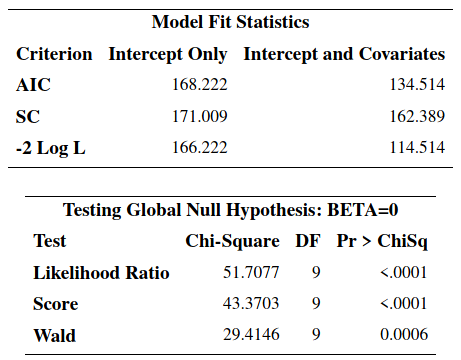
\includegraphics[width=0.55\textwidth]{img/c4/slides8-e11}
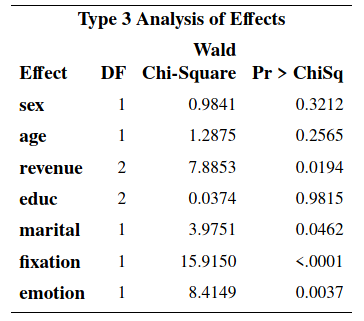
\includegraphics[width=0.44\textwidth]{img/c4/slides8-e12}
\end{center}
{\small 
\bi \item Goodness of fit diagnostics are given for the fitted model and the null model in which the probability of success is constant (Intercept Only). 
\item In addition to information criteria, likelihood tests (Wald, score, likelihood ratio) are given for testing the global null hypothesis of significance, $\Hy_0: \beta_1 = \cdots = \beta_p = 0$.
\item Parameter significance (Type III effects) is based on Wald statistics (for likelihood ratio, use the \texttt{genmod} procedure with option \texttt{type3}).
\ei
}
\end{frame}
\begin{frame}
\frametitle{Parameter estimates}
\begin{center}
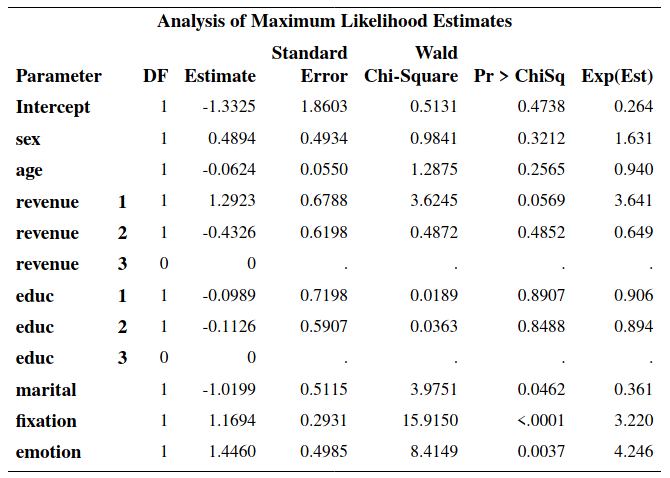
\includegraphics[width = 0.85\textwidth]{img/c4/slides8-e13}
\end{center}
{\footnotesize 

\bi
\item The option \code{expb} will provide each of the $\exp(\hat{\beta}_j)$ values in the last column.
\item The tests of significance are Wald-based.
\ei
}
\end{frame}

\begin{frame}
 \frametitle{Table of coefficients}
 \begin{center}
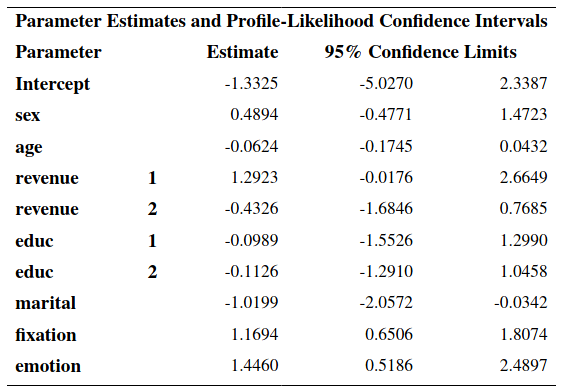
\includegraphics[width = 0.8\linewidth]{img/c4/slides8-e14.png}
\end{center}
\end{frame}
\begin{frame}{Table of exponentiated coefficients}
\begin{center}
 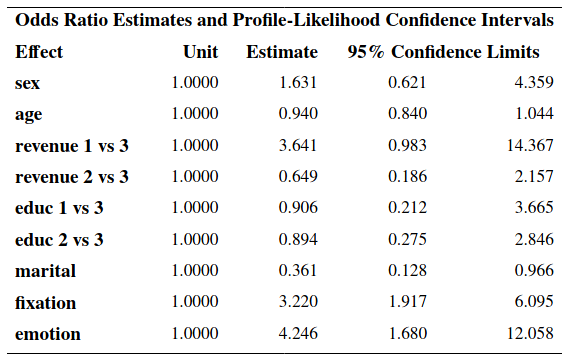
\includegraphics[width = 0.8\linewidth]{img/c4/slides8-e15.png}
\end{center}
\begin{footnotesize}
 \bi 
 \item On the exponentiated scale, the parameter is not significant at level 5\% if $1$ is in the confidence interval.
 \item To obtain likelihood-ratio based confidence intervals, use option \texttt{plrl}.
 \ei
\end{footnotesize}




\end{frame}

\begin{frame}[fragile]
\frametitle{Parameter interpretations}
\bi
\item $\exp(\hat{\beta}_{\code{sex}})=1.631$: the odds of buying for women (\code{sex=1}) is $1.631$ times higher than for men, \textbf{when all other variables in the model are held constant}. Therefore, women have a higher chance of buying than men, even after adjusting for all the other variables. 
\item $\exp(\hat{\beta}_{\code{age}})=0.94$: when age increases by one year, the odds of buying change by a factor of $0.94$, i.e. decreases by $6\%$, \textbf{when all other variables in the model are held constant}. 
%when age increases by one year, the odds of buying is multiplied by 0.894 (or divided by 1/0.89=1.12) \textbf{when all other variables in the model are held constant}.
\item $\exp(\hat{\beta}_{\code{fixation}})=3.22$: when fixation time increases by one second the odds of buying is multiplied by $3.22$  \textbf{when all other variables in the model are held constant}.  

\ei
\end{frame}
\begin{frame}[fragile]
\frametitle{Comparing the levels of \code{revenue}}
\bi
\item The coefficient for $\code{revenu}_1$ is relative to \code{revenu=3} and $\exp(\hat{\beta}_{\code{revenu}_1})=3.641$:  the estimated odds of buying for low-income individuals (\code{revenue=1}) is $3.641$ times the odds of buying for high-income individuals (\code{revenue=3}), \textbf{when all other variables in the model are held constant}. 
\item To get the odds ratio between levels $1$ and $2$ of \code{revenue}, we would need to fit another model, changing the reference category.
\item We could also easily do it by hand: $3.641/0.649=5.61$ implies that the odds for revenue level $1$ are $461\%$ higher than the odds for revenue level $2$, when all other variables are held constant.
\ei
\end{frame}

% \begin{frame}{Note on profile-based confidence intervals}
% \bi
% \item The confidence intervals are based on a profile likelihood (akin to likelihood ratio test). 
% \bi \item They are therefore \textbf{invariant to reparametrization} of the model, so you can get a confidence interval for $\exp(\beta_k)$ by exponentiating the limits of the confidence interval for $\beta_k$ (try with the previous tables).
% 
% \item The confidence intervals are \textbf{asymmetric}.
% \ei
% 
% \ei
% \end{frame}

\begin{frame}[fragile]
\frametitle{Visual representation of the odds ratios}
\begin{center}
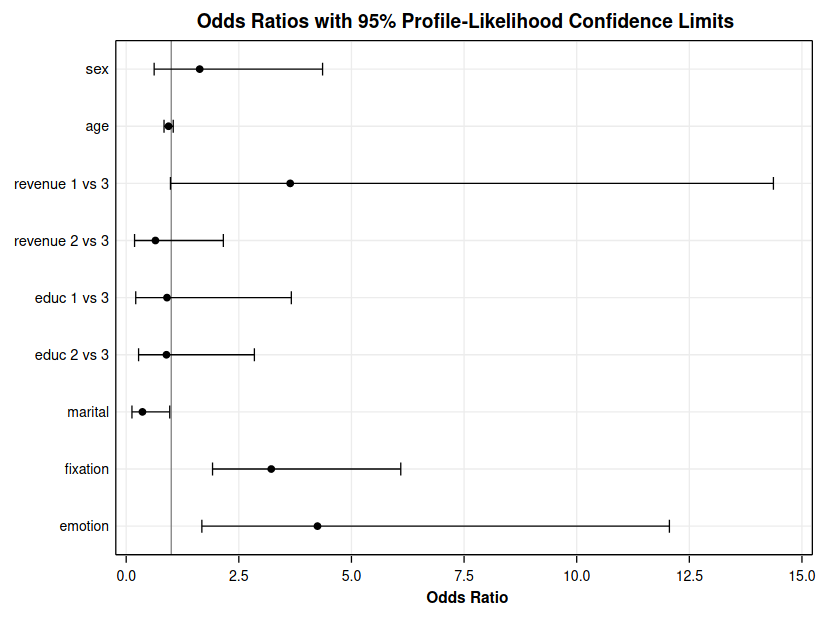
\includegraphics[width = 0.8\linewidth]{img/c4/slides8-e16}

\end{center}
{\footnotesize 


The confidence intervals are based on a profile likelihood.
They are therefore \textbf{invariant to reparametrization} of the model, so you can get a confidence interval for $\exp(\beta_k)$ by exponentiating the limits of the confidence interval for $\beta_k$.

}
\end{frame}


\end{document}
